\documentclass[xcolor=dvipsnames]{beamer} 
\usepackage{natbib}                 % fancy bibliography.
\usepackage{url}                    % allow printing of urls.
\usepackage{dsfont}
\usepackage{amsmath}
\usepackage{wrapfig}
\usepackage{epstopdf}
\usepackage{listings}

\usepackage{color}

\usepackage{caption}
\setbeamertemplate{footline}[frame number]
\captionsetup{font=scriptsize,labelfont=bf}


\title{\textbf{An introduction to Python}}

\date{}


\definecolor{dkgreen}{rgb}{0,0.6,0}
\definecolor{gray}{rgb}{0.5,0.5,0.5}
\definecolor{mauve}{rgb}{0.58,0,0.82}

\lstset{frame=tb,
  language=Python,
  aboveskip=3mm,
  belowskip=3mm,
  showstringspaces=false,
  columns=flexible,
  basicstyle={\small},
  numbers=none,
  numberstyle=\tiny\color{gray},
  keywordstyle=\color{blue},
  commentstyle=\color{dkgreen},
  stringstyle=\color{mauve},
  breaklines=true,
  breakatwhitespace=true
  tabsize=3
}

\begin{document}
\lstset{language=Python}

\begin{frame}[t]
  \maketitle
  \vskip -9em
\end{frame}

\AtBeginSection[] % Do nothing for \section*
{ 
  \frame<beamer>
    {
          \frametitle{Contents}
	        \tableofcontents[current]
	}
}



\section{Why Python?}

\begin{frame}
\frametitle{Our needs}

\begin{itemize}
\item Get data (simulation, experiment control)
\item Manipulate and process data.
\item Visualize results... to understand what we are doing!
\end{itemize}

\end{frame}


\begin{frame}
\frametitle{What is programming?}

\begin{figure}
\begin{center}
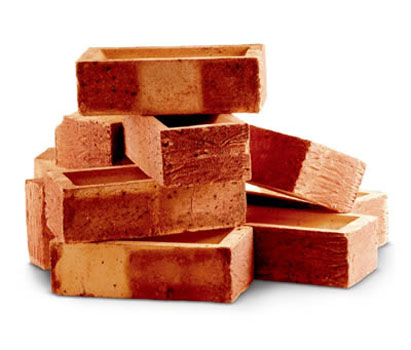
\includegraphics{images/bricks.jpg}
\end{center}
\end{figure}
\end{frame}


\begin{frame}
\frametitle{Why Python?}
\begin{itemize}
\item Readable and well structured language
\item Quick development and execution time
\item Rich collections of existing bricks
\end{itemize}
\end{frame}

\section{The basics}

\begin{frame}
\begin{block}{Value or object}
\frametitle{Values and Data Types}
A \textbf{value} (or an \textbf{object}) is one of the fundamental thing that
a program manipulates. Objects are classified into different \textbf{types} or
\textbf{class}.
\end{block}

\vspace{1em}
\lstinputlisting[language=Python]{src/values.py}
\end{frame}

\begin{frame}
\frametitle{Data Types}

\begin{tabular}{l | l}
boolean & \texttt{True} \\
string & \texttt{"Hello world"} \\
integer & \texttt{5} \\
float & \texttt{1.} \\ 
complex & \texttt{1 + 1j}
\end{tabular}

\vspace{1em}
\begin{alertblock}{Question}
\begin{itemize}
\item What is the type of the following values: "3", '5' ?
\end{itemize}
\end{alertblock}
\end{frame}

\begin{frame}
\frametitle{Using Python as a calculator}

The \textbf{interpreter} can be used as a simple calculator.

\vspace{1em}
\lstinputlisting[language=Python]{src/calculator.py}

\vspace{1em}
\begin{alertblock}{Question}
\begin{itemize}
\item Do you understand all the outputs?
\item What do you think the pound (\texttt{\#}) sign means?
\end{itemize}
\end{alertblock}

\end{frame}

\begin{frame}
\frametitle{Variables and assignments}
\begin{block}{Variables}

A \textbf{variable} is a name that refers to a value.
A value is \textbf{assigned} to a variable.
\end{block}
\vspace{1em}
\lstinputlisting[language=Python]{src/variables.py}

\vspace{1em}
\begin{alertblock}{Question}
\begin{itemize}
\item What are the types of \texttt{a} and \texttt{b}?
\item What is the type of \texttt{c}?
\end{itemize}
\end{alertblock}
\end{frame}

\begin{frame}
\frametitle{Variable names and keywords}
\end{frame}

\begin{frame}
\frametitle{Exercises}
\begin{itemize}
\item \textbf{Q1} What is printed when the following statements are executed?
\lstinputlisting{src/Q01.py}
\item \textbf{Q2} How would you swap the values of two variables \texttt{a}
and \texttt{b}?
\end{itemize}
\end{frame}


\end{document}
